
\section{Grafos UF}

\begin{table}[htb]
\centering
\caption{Variação percentual das métricas de redes mês a mês para o grafo de UFs (Parte 1)}
\label{tab:metricas-redes-pandemia:grafo-mensal-por-uf1}
\begin{tabular}{l|rrrr}
\toprule
Mês & Densidade & Transitividade & Grau médio & \shortstack{Grau médio\\ponderado} \\
\midrule
01/2019 & - & - & - & - \\
02/2019 &  0.54\% &  0.55\% &  0.54\% &  9.88\% \\
03/2019 &  0.00\% &  0.17\% &  0.00\% & 25.54\% \\
04/2019 &  0.54\% &  0.57\% &  0.54\% & 23.86\% \\
05/2019 &  0.81\% &  0.81\% &  0.81\% & 36.91\% \\
06/2019 &  0.27\% &  0.32\% &  0.27\% & 23.88\% \\
07/2019 &  0.54\% &  0.57\% &  0.54\% & 28.36\% \\
08/2019 &  0.54\% &  0.57\% &  0.54\% & 35.37\% \\
09/2019 &  0.27\% &  0.36\% &  0.27\% & 32.62\% \\
10/2019 &  0.81\% &  0.82\% &  0.81\% & 42.89\% \\
11/2019 &  0.27\% &  0.34\% &  0.27\% & 43.93\% \\
12/2019 &  0.27\% &  0.36\% &  0.27\% & 29.66\% \\
01/2020 &  0.81\% &  0.83\% &  0.81\% & 28.84\% \\
02/2020 &  0.27\% &  0.44\% &  0.27\% & 32.22\% \\
03/2020 &  0.54\% &  0.59\% &  0.54\% & 36.09\% \\
04/2020 & -0.27\% & -0.07\% & -0.27\% & -7.91\% \\
05/2020 & -0.27\% & -0.18\% & -0.27\% & 12.47\% \\
06/2020 &  0.00\% &  0.11\% &  0.00\% & 34.61\% \\
07/2020 &  0.54\% &  0.57\% &  0.54\% & 62.51\% \\
08/2020 &  0.54\% &  0.59\% &  0.54\% & 55.16\% \\
09/2020 &  1.08\% &  1.09\% &  1.08\% & 60.32\% \\
10/2020 &  0.00\% &  0.17\% &  0.00\% & 61.19\% \\
\bottomrule
\end{tabular}
\fdadospesquisa
\end{table}

\begin{table}[htb]
\centering
\caption{Variação das métricas de redes mês a mês para o grafo de UFs (Parte 2)}
\label{tab:metricas-redes-pandemia:grafo-mensal-por-uf2}
\begin{tabular}{l|rrrr}
\toprule
Mês & \shortstack{Assortatividade\\de grau} & \shortstack{Assortatividade\\de região} & \shortstack{Caminho mínimo\\médio} & \shortstack{Caminho mínimo\\médio ponderado} \\
\midrule
01/2019 & - & - & - & - \\
02/2019 & -15.60\% & -50.13\% & -0.55\% &  -8.47\% \\
03/2019 &   0.05\% &  -0.00\% &  0.00\% & -25.12\% \\
04/2019 &   7.91\% & -15.39\% & -0.55\% & -22.23\% \\
05/2019 & -31.31\% & -85.53\% & -0.83\% & -25.07\% \\
06/2019 &  21.99\% &  13.35\% & -0.27\% &   2.44\% \\
07/2019 & -17.07\% & -57.33\% & -0.55\% &  -1.69\% \\
08/2019 &   7.91\% & -57.33\% & -0.55\% & -11.02\% \\
09/2019 &   4.73\% & -28.82\% & -0.27\% &  -2.55\% \\
10/2019 &  -6.87\% & -43.83\% & -0.83\% & -11.15\% \\
11/2019 &   8.56\% &  13.35\% & -0.27\% & -14.48\% \\
12/2019 &   4.73\% & -70.86\% & -0.27\% &   2.50\% \\
01/2020 & -25.43\% & -43.83\% & -0.83\% &   1.69\% \\
02/2020 & -18.97\% & -28.82\% & -0.27\% &  -5.58\% \\
03/2020 &  -7.22\% & -15.39\% & -0.55\% &  -4.69\% \\
04/2020 &   1.98\% & -13.38\% &  0.27\% &  36.70\% \\
05/2020 &  37.79\% &  29.14\% &  0.27\% &   2.72\% \\
06/2020 &  19.66\% & -42.28\% &  0.00\% & -15.66\% \\
07/2020 &   7.91\% & -15.39\% & -0.55\% & -32.97\% \\
08/2020 &  -7.22\% & -15.39\% & -0.55\% & -35.56\% \\
09/2020 & -16.88\% & -71.96\% & -1.11\% & -37.64\% \\
10/2020 &   0.05\% & -42.28\% &  0.00\% & -30.06\% \\
\bottomrule
\end{tabular}
\fdadospesquisa
\end{table}

\begin{table}[htb]
\centering
\caption{Variação das métricas de rede a cada trimestre para o grafo de UFs (Parte 1)}
\label{tab:metricas-redes-pandemia:grafo-trimestral-por-uf1}
\begin{tabular}{l|rrrr}
\toprule
Mês & Densidade & Transitividade & Grau médio & \shortstack{Grau médio\\ponderado} \\
\midrule
2020/1 & - & - & - & - \\
2020/2 & -0.80\% & -0.78\% & -0.80\% & -14.60\% \\
2020/3 &  0.27\% &  0.22\% &  0.27\% &  20.35\% \\
\bottomrule
\end{tabular}
\fdadospesquisa
\end{table}

\begin{table}[htb]
\centering
\caption{Variação das métricas de rede a cada trimestre para o grafo de UFs (Parte 2)}
\label{tab:metricas-redes-pandemia:grafo-trimestral-por-uf2}
\begin{tabular}{l|rrrr}
\toprule
Mês & \shortstack{Assortatividade\\de grau} & \shortstack{Assortatividade\\de região} & \shortstack{Caminho mínimo\\médio} & \shortstack{Caminho mínimo\\médio ponderado} \\
\midrule
2020/1 & - & - & - & - \\
2020/2 &  77.29\% &   1.84\% &  0.85\% &   6.63\% \\
2020/3 & -34.35\% & -83.36\% & -0.28\% & -33.74\% \\
\bottomrule
\end{tabular}
\fdadospesquisa
\end{table}

\begin{table}[htb]
\centering
\caption{Diferença entre as métricas de rede para UFs afetadas e não afetadas}
\label{tab:metricas-redes-pandemia:diferenca-afetadas-por-uf}
\begin{tabular}{l|rrrrrrr}
\toprule
Métrica & Média & \shortstack{Desvio\\padrão} & Mínimo & P25 & Mediana & P75 & Máximo \\
\midrule
Grau médio                     & -1.85\% &   2.51\% &  -0.26\% & -3.70\% &  0.00\% &  0.00\% &    0.00\% \\ \hline
\shortstack[l]{Coeficiente de\\agrupamento}     &  0.33\% &   4.71\% &   2.79\% & -2.34\% & -0.83\% &  6.67\% &  -14.51\% \\ \hline
Excentricidade                 & -4.17\% & -20.41\% &   0.00\% &  0.00\% &  0.00\% &  0.00\% & -100.00\% \\ \hline
\shortstack[l]{Caminho mínimo\\médio}           &  1.85\% &   2.46\% &   0.00\% &  0.00\% &  0.00\% &  3.70\% &   -0.28\% \\ \hline
\shortstack[l]{Caminho mínimo\\médio ponderado} & -6.58\% &   0.14\% &  -2.01\% & -7.36\% & -0.36\% & -1.03\% &  -37.83\% \\ \hline
\shortstack[l]{Centralidade de\\proximidade}    & -1.71\% &   2.28\% &   0.25\% & -3.45\% &  0.00\% &  0.00\% &    0.00\% \\ \hline
\shortstack[l]{Centralidade de\\informação}     & -1.07\% &  -1.71\% &   9.93\% & -1.09\% &  0.16\% &  0.10\% &   -8.60\% \\ \hline
\shortstack[l]{Centralidade de\\autovalor}      & -3.84\% &  -1.85\% &  23.00\% & -0.99\% & -1.58\% & -4.25\% &  -20.99\% \\ \hline
\shortstack[l]{Centralidade de\\intermediação}  &  - &     - & 206.06\% &  0.00\% &  0.00\% &  0.00\% &    - \\ \hline
PageRank                       & -0.63\% &   0.02\% &   4.37\% & -1.23\% & -1.61\% & -1.01\% &   -5.26\% \\
\bottomrule
\end{tabular}
\fdadospesquisa
\end{table}

\section{Grafos Seção}

\begin{table}[htb]
\centering
\caption{Variação percentual das métricas de redes mês a mês para o grafo de seções (Parte 1)}
\label{tab:metricas-redes-pandemia:grafo-mensal-por-secao1}
\begin{tabular}{l|rrrr}
\toprule
Mês & Densidade & Transitividade & Grau médio & \shortstack{Grau médio\\ponderado} \\
\midrule
01/2019 &  - &  - &  - &  - \\
02/2019 & -0.57\% & -0.55\% & -0.57\% &  9.89\%\\
03/2019 &  0.57\% &  0.31\% &  0.57\% & 25.54\%\\
04/2019 & -1.15\% & -1.20\% & -1.15\% & 23.86\%\\
05/2019 &  1.15\% &  0.15\% &  1.15\% & 36.92\%\\
06/2019 & -1.72\% & -1.33\% & -1.72\% & 23.89\%\\
07/2019 & -0.57\% & -1.00\% & -0.57\% & 28.37\%\\
08/2019 & -0.57\% & -0.63\% & -0.57\% & 35.37\%\\
09/2019 &  0.00\% &  0.18\% &  0.00\% & 32.63\%\\
10/2019 & -0.57\% &  0.13\% & -0.57\% & 42.89\%\\
11/2019 & -1.72\% & -1.25\% & -1.72\% & 43.94\%\\
12/2019 &  1.15\% &  0.85\% &  1.15\% & 29.66\%\\
01/2020 &  2.30\% &  1.87\% &  2.30\% & 28.85\%\\
02/2020 &  1.15\% &  0.46\% &  1.15\% & 32.22\%\\
03/2020 &  1.72\% &  0.98\% &  1.72\% & 36.10\%\\
04/2020 & -0.57\% & -0.38\% & -0.57\% & -7.92\%\\
05/2020 & -0.57\% & -0.47\% & -0.57\% & 12.47\%\\
06/2020 & -1.72\% & -0.72\% & -1.72\% & 34.62\%\\
07/2020 & -1.72\% & -1.97\% & -1.72\% & 62.52\%\\
08/2020 &  0.00\% & -0.15\% &  0.00\% & 55.16\%\\
09/2020 &  1.72\% &  1.24\% &  1.72\% & 60.33\%\\
10/2020 &  0.00\% & -0.60\% &  0.00\% & 61.20\%\\
\bottomrule
\end{tabular}
\fdadospesquisa
\end{table}

\begin{table}[htb]
\centering
\caption{Variação das métricas de redes mês a mês para o grafo de seções (Parte 2)}
\label{tab:metricas-redes-pandemia:grafo-mensal-por-secao2}
\begin{tabular}{l|rrrr}
\toprule
Mês & \shortstack{Assortatividade\\de grau} & \shortstack{Assortatividade\\de seção} & \shortstack{Caminho mínimo\\médio} & \shortstack{Caminho mínimo\\médio ponderado} \\
\midrule
01/2019 &  - &  - &  - &  - \\
02/2019 &   2.76\% &  -4.38\% &  0.45\% &  29.22\% \\
03/2019 &  -9.42\% &   2.43\% & -0.45\% & -11.35\% \\
04/2019 &   4.86\% &  -8.49\% &  0.90\% &   2.19\% \\
05/2019 &   1.47\% & -55.07\% & -0.45\% &   3.75\% \\
06/2019 &  16.41\% &  51.81\% &  0.90\% &   5.20\% \\
07/2019 &   1.48\% &  -6.63\% &  0.45\% & -15.91\% \\
08/2019 &   6.16\% &  -4.75\% &  0.45\% & -13.54\% \\
09/2019 &  -5.13\% &  61.37\% & -0.45\% & -10.76\% \\
10/2019 &  -1.58\% &  59.27\% &  0.00\% & -15.12\% \\
11/2019 &  10.43\% &  50.66\% &  0.90\% & -38.71\% \\
12/2019 &  -3.53\% &   8.42\% & -0.90\% & -41.20\% \\
01/2020 & -14.48\% &  16.07\% & -1.80\% & -25.39\% \\
02/2020 &  -1.24\% & -53.98\% & -0.45\% & -36.64\% \\
03/2020 &  -7.40\% & -50.23\% & -0.90\% &  22.58\% \\
04/2020 &  -4.91\% &  -5.13\% &  0.45\% &  28.02\% \\
05/2020 &  -8.57\% &  -6.63\% &  0.45\% & 114.33\% \\
06/2020 &  -3.99\% & -11.95\% &  1.35\% &  72.81\% \\
07/2020 &  -4.68\% & -80.36\% &  1.80\% &  65.47\% \\
08/2020 & -11.69\% & -64.36\% &  0.45\% &  60.28\% \\
09/2020 & -10.17\% & -49.15\% & -0.90\% &  56.97\% \\
10/2020 &  -6.61\% & -65.48\% &  0.45\% & -33.58\% \\
\bottomrule
\end{tabular}
\fdadospesquisa
\end{table}

\begin{table}[htb]
\centering
\caption{Variação das métricas de rede a cada trimestre para o grafo de seções (Parte 1)}
\label{tab:metricas-redes-pandemia:grafo-trimestral-por-secao1}
\begin{tabular}{l|rrrr}
\toprule
Mês & Densidade & Transitividade & Grau médio & \shortstack{Grau médio\\ponderado} \\
\midrule
2020/1 & - & - & - & - \\
2020/2 & -1.66\% & -0.92\% & -1.66\% & -14.60\% \\
2020/3 & -1.10\% & -0.59\% & -1.10\% &  20.35\% \\
\bottomrule
\end{tabular}
\fdadospesquisa
\end{table}

\begin{table}[htb]
\centering
\caption{Variação das métricas de rede a cada trimestre para o grafo de seções (Parte 2)}
\label{tab:metricas-redes-pandemia:grafo-trimestral-por-secao2}
\begin{tabular}{l|rrrr}
\toprule
Mês & \shortstack{Assortatividade\\de grau} & \shortstack{Assortatividade\\de seção} & \shortstack{Caminho mínimo\\médio} & \shortstack{Caminho mínimo\\médio ponderado} \\
\midrule
2020/1 & - & - & - & - \\
2020/2 & 11.16\% &  72.34\% & 0.93\% & 122.98\% \\
2020/3 & -2.87\% & -12.77\% & 0.93\% & 100.19\% \\
\bottomrule
\end{tabular}
\fdadospesquisa
\end{table}

\begin{table}[htb]
\centering
\caption{Diferença entre as métricas de rede para seções afetadas e não afetadas}
\label{tab:metricas-redes-pandemia:diferenca-afetadas-por-secao}
\begin{tabular}{l|rrrrrrr}
\toprule
Métrica & Média & \shortstack{Desvio\\padrão} & Mínimo & P25 & Mediana & P75 & Máximo \\
\midrule
Grau médio                     &  0.02\% & -0.04\% & 0.11\% & 0.05\% &  0.00\% &  0.00\% & -0.05\% \\ \hline
\shortstack[l]{Coeficiente de\\agrupamento}     &  0.16\% & -0.01\% & 0.38\% & 0.15\% &  0.11\% &  0.14\% &  0.07\% \\ \hline
Excentricidade                 &  0.00\% &  0.00\% & 0.00\% & 0.00\% &  0.00\% &  0.00\% &  0.00\% \\ \hline
\shortstack[l]{Caminho mínimo\\médio}           & -0.01\% & -0.03\% & 0.05\% & 0.00\% &  0.00\% & -0.04\% & -0.05\% \\ \hline
\shortstack[l]{Caminho mínimo\\médio ponderado} &  0.00\% & -0.00\% & 0.00\% & 0.00\% & -0.00\% & -0.00\% & -0.00\% \\ \hline
\shortstack[l]{Centralidade de\\proximidade}    &  0.01\% & -0.03\% & 0.05\% & 0.04\% &  0.00\% &  0.00\% & -0.05\% \\ \hline
\shortstack[l]{Centralidade de\\informação}     &  0.00\% & -0.00\% & 0.00\% & 0.00\% &  0.00\% & -0.00\% & -0.00\% \\ \hline
\shortstack[l]{Centralidade de\\autovalor}      &  0.32\% & -0.00\% & 0.56\% & 0.39\% &  0.20\% &  0.25\% &  0.28\% \\ \hline
\shortstack[l]{Centralidade de\\intermediação}  &  0.43\% &  0.12\% & 0.76\% & 0.34\% &  0.00\% &  0.46\% &  0.00\% \\ \hline
PageRank                       &  0.07\% & -0.04\% & 0.17\% & 0.07\% &  0.08\% &  0.11\% & -0.21\% \\
\bottomrule
\end{tabular}
\fdadospesquisa
\end{table}

\section{Grafos CNAE}

\begin{table}[htb]
\centering
\caption{Variação percentual das métricas de redes mês a mês para o grafo de CNAEs (Parte 1)}
\label{tab:metricas-redes-pandemia:grafo-mensal-por-cnae1}
\begin{tabular}{l|rrrr}
\toprule
Mês & Densidade & Transitividade & Grau médio & \shortstack{Grau médio\\ponderado} \\
\midrule
01/2019 & - & - & - & - \\
02/2019 &  4.35\% &  1.75\% &  4.45\% &  9.79\% \\
03/2019 &  5.96\% &  2.29\% &  6.15\% & 25.32\% \\
04/2019 &  9.60\% &  3.67\% &  9.70\% & 23.75\% \\
05/2019 & 11.46\% &  4.22\% & 11.66\% & 36.67\% \\
06/2019 &  7.55\% &  2.71\% &  7.55\% & 23.89\% \\
07/2019 & 12.16\% &  4.16\% & 12.06\% & 28.48\% \\
08/2019 & 12.70\% &  4.64\% & 12.80\% & 35.25\% \\
09/2019 & 11.38\% &  4.45\% & 11.48\% & 32.51\% \\
10/2019 & 13.87\% &  5.36\% & 14.27\% & 42.38\% \\
11/2019 & 12.57\% &  4.84\% & 12.67\% & 43.81\% \\
12/2019 &  6.15\% &  2.35\% &  6.62\% & 29.09\% \\
01/2020 &  9.87\% &  3.64\% & 10.27\% & 28.39\% \\
02/2020 &  8.58\% &  3.01\% &  8.87\% & 31.87\% \\
03/2020 &  9.29\% &  3.80\% &  9.68\% & 35.62\% \\
04/2020 & -2.40\% & -0.24\% & -2.40\% & -7.92\% \\
05/2020 &  1.98\% &  1.67\% &  2.07\% & 12.37\% \\
06/2020 &  7.94\% &  3.99\% &  8.13\% & 34.38\% \\
07/2020 & 11.86\% &  5.21\% & 12.46\% & 61.65\% \\
08/2020 & 10.99\% &  4.48\% & 10.89\% & 55.30\% \\
09/2020 &  9.68\% &  4.69\% & 10.26\% & 59.47\% \\
10/2020 &  7.63\% &  3.96\% &  8.02\% & 60.62\% \\
\bottomrule
\end{tabular}
\fdadospesquisa
\end{table}

\begin{table}[htb]
\centering
\caption{Variação das métricas de redes mês a mês para o grafo de CNAEs (Parte 2)}
\label{tab:metricas-redes-pandemia:grafo-mensal-por-cnae2}
\begin{tabular}{l|rrrr}
\toprule
Mês & \shortstack{Assortatividade\\de grau} & \shortstack{Assortatividade\\de seção} & \shortstack{Caminho mínimo\\médio} & \shortstack{Caminho mínimo\\médio ponderado} \\
\midrule
01/2019 & - & - & - & - \\
02/2019 &  0.38\% &  -6.76\% & -0.72\% &  -9.37\% \\
03/2019 &  1.52\% & -22.04\% & -0.93\% &  35.22\% \\
04/2019 &  1.80\% &  -8.60\% & -1.49\% &  33.50\% \\
05/2019 &  2.69\% & -23.49\% & -1.83\% & -13.22\% \\
06/2019 &  1.02\% & -24.50\% & -1.15\% & -15.84\% \\
07/2019 &  1.76\% &   4.38\% & -1.77\% & -17.73\% \\
08/2019 &  1.77\% & -16.28\% & -1.64\% &   3.81\% \\
09/2019 &  0.86\% &   3.95\% & -1.65\% & -29.89\% \\
10/2019 &  1.55\% &  -4.69\% & -1.83\% & -35.86\% \\
11/2019 &  1.02\% &  -8.01\% & -1.83\% & -36.74\% \\
12/2019 &  0.52\% & -10.46\% & -1.08\% & -30.56\% \\
01/2020 &  2.06\% &  -6.52\% & -1.50\% & -28.02\% \\
02/2020 &  1.27\% &   9.35\% & -1.30\% & -23.95\% \\
03/2020 &  1.61\% &   1.73\% & -1.40\% & -23.14\% \\
04/2020 & -0.02\% &   8.10\% &  0.58\% &  -8.54\% \\
05/2020 &  1.14\% &  16.10\% & -0.27\% &   9.73\% \\
06/2020 &  2.35\% &   0.88\% & -1.13\% &  16.51\% \\
07/2020 &  3.60\% &  15.25\% & -1.66\% &   1.86\% \\
08/2020 &  1.83\% &  12.58\% & -1.57\% & -26.79\% \\
09/2020 &  2.24\% &  16.47\% & -1.21\% &   5.56\% \\
10/2020 &  1.30\% &  -4.01\% & -0.98\% & -17.64\% \\
\bottomrule
\end{tabular}
\fdadospesquisa
\end{table}

\begin{table}[htb]
\centering
\caption{Variação das métricas de rede a cada trimestre para o grafo de CNAEs (Parte 1)}
\label{tab:metricas-redes-pandemia:grafo-trimestral-por-cnae1}
\begin{tabular}{l|rrrr}
\toprule
Mês & Densidade & Transitividade & Grau médio & \shortstack{Grau médio\\ponderado} \\
\midrule
2020/1 & - & - & - & - \\
2020/2 & -4.91\% & -1.09\% & -4.91\% & -14.60\% \\
2020/3 &  0.82\% &  0.98\% &  0.91\% &  20.25\% \\
\bottomrule
\end{tabular}
\fdadospesquisa
\end{table}

\begin{table}[htb]
\centering
\caption{Variação das métricas de rede a cada trimestre para o grafo de CNAEs (Parte 2)}
\label{tab:metricas-redes-pandemia:grafo-trimestral-por-cnae2}
\begin{tabular}{l|rrrr}
\toprule
Mês & \shortstack{Assortatividade\\de grau} & \shortstack{Assortatividade\\de seção} & \shortstack{Caminho mínimo\\médio} & \shortstack{Caminho mínimo\\médio ponderado} \\
\midrule
2020/1 & - & - & - & - \\
2020/2 & -0.21\% & 8.07\% & 0.98\% & 71.35\% \\
2020/3 &  0.66\% & 3.81\% & 0.05\% & 26.02\% \\
\bottomrule
\end{tabular}
\fdadospesquisa
\end{table}

\begin{table}[htb]
\centering
\caption{Diferença entre as métricas de rede para CNAEs afetadas e não afetadas}
\label{tab:metricas-redes-pandemia:diferenca-afetadas-por-cnae}
\begin{tabular}{l|rrrrrrr}
\toprule
Métrica & Média & \shortstack{Desvio\\padrão} & Mínimo & P25 & Mediana & P75 & Máximo \\
\midrule
Grau médio                     &  0.02\% & -0.04\% & 0.11\% & 0.05\% &  0.00\% &  0.00\% & -0.05\% \\ \hline
\shortstack[l]{Coeficiente de\\agrupamento}     &  0.16\% & -0.01\% & 0.38\% & 0.15\% &  0.11\% &  0.14\% &  0.07\% \\ \hline
Excentricidade                 &  0.00\% &  0.00\% & 0.00\% & 0.00\% &  0.00\% &  0.00\% &  0.00\% \\ \hline
\shortstack[l]{Caminho mínimo\\médio}           & -0.01\% & -0.03\% & 0.05\% & 0.00\% &  0.00\% & -0.04\% & -0.05\% \\ \hline
\shortstack[l]{Caminho mínimo\\médio ponderado} &  0.00\% & -0.00\% & 0.00\% & 0.00\% & -0.00\% & -0.00\% & -0.00\% \\ \hline
\shortstack[l]{Centralidade de\\proximidade}    &  0.01\% & -0.03\% & 0.05\% & 0.04\% &  0.00\% &  0.00\% & -0.05\% \\ \hline
\shortstack[l]{Centralidade de\\informação}     &  0.00\% & -0.00\% & 0.00\% & 0.00\% &  0.00\% & -0.00\% & -0.00\% \\ \hline
\shortstack[l]{Centralidade de\\autovalor}      &  0.32\% & -0.00\% & 0.56\% & 0.39\% &  0.20\% &  0.25\% &  0.28\% \\ \hline
\shortstack[l]{Centralidade de\\intermediação}  &  0.43\% &  0.12\% & 0.76\% & 0.34\% &  0.00\% &  0.46\% &  0.00\% \\ \hline
PageRank                       &  0.07\% & -0.04\% & 0.17\% & 0.07\% &  0.08\% &  0.11\% & -0.21\% \\
\bottomrule
\end{tabular}
\fdadospesquisa
\end{table}

\section{Classificação UF}

\begin{figure}[htb] 
    \centering 
    \caption{PCA sobre dados mensais de UFs}
    \label{fig:resultados:base-de-dados-24-pca-monthly-uf} 
    \begin{subfigure}[b]{0.45\textwidth}
        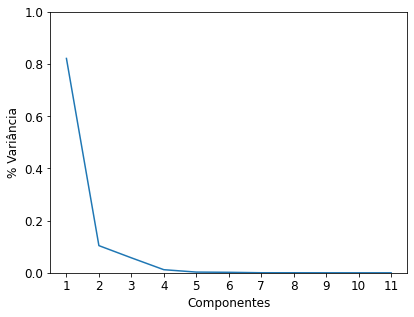
\includegraphics[scale=0.45]{images/base-de-dados-24.1-pca-components-monthly-uf.png}
        \caption{Percentual de variância explicada de cada componente principal}
        \label{fig:resultados:base-de-dados-24.1-pca-components-monthly-uf}
    \end{subfigure} ~ \quad
    \begin{subfigure}[b]{0.45\textwidth}
        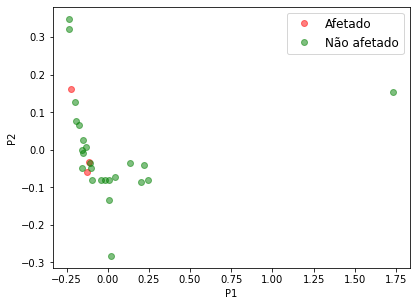
\includegraphics[scale=0.45]{images/base-de-dados-24.2-pca-2d-monthly-uf.png}
        \caption{Visualização dos dados projetados sobre as duas componentes principais}
        \label{fig:resultados:base-de-dados-24.2-pca-2d-monthly-uf}
    \end{subfigure}
    \fdadospesquisa
\end{figure}

\begin{figure}[htb] 
    \centering 
    \caption{PCA sobre dados totais de UFs}
    \label{fig:resultados:base-de-dados-25-pca-2d-total-uf} 
    \begin{subfigure}[b]{0.45\textwidth}
        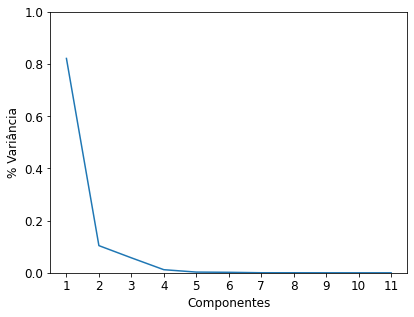
\includegraphics[scale=0.45]{images/base-de-dados-25.1-pca-components-total-uf.png}
        \caption{Percentual de variância explicada de cada componente principal}
        \label{fig:resultados:base-de-dados-25.1-pca-components-total-uf}
    \end{subfigure} ~ \quad
    \begin{subfigure}[b]{0.45\textwidth}
        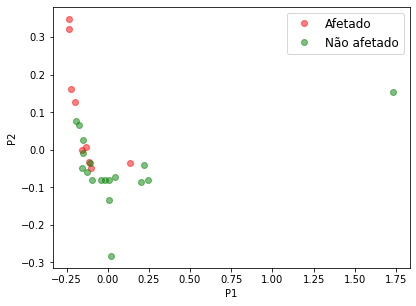
\includegraphics[scale=0.45]{images/base-de-dados-25.2-pca-2d-total-uf.png}
        \caption{Visualização dos dados projetados sobre as duas componentes principais}
        \label{fig:resultados:base-de-dados-25.2-pca-2d-total-uf}
    \end{subfigure}
    \fdadospesquisa
\end{figure}

\section{Classificação Seção}

\begin{figure}[htb] 
    \centering 
    \caption{PCA sobre dados mensais de seções}
    \label{fig:resultados:base-de-dados-26-pca-components-monthly-secao} 
    \begin{subfigure}[b]{0.45\textwidth}
        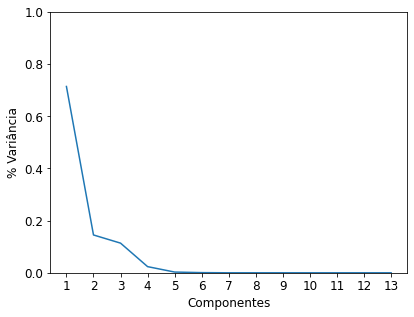
\includegraphics[scale=0.45]{images/base-de-dados-26.1-pca-components-monthly-secao.png}
        \caption{Percentual de variância explicada de cada componente principal}
        \label{fig:resultados:26.1-pca-components-monthly-seca}
    \end{subfigure} ~ \quad
    \begin{subfigure}[b]{0.45\textwidth}
        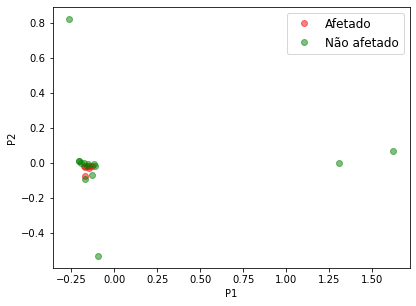
\includegraphics[scale=0.45]{images/base-de-dados-26.2-pca-2d-monthly-secao.png}
        \caption{Visualização dos dados projetados sobre as duas componentes principais}
        \label{fig:resultados:base-de-dados-26.2-pca-2d-monthly-secao}
    \end{subfigure}
    \fdadospesquisa
\end{figure}

\begin{figure}[htb] 
    \centering 
    \caption{PCA sobre dados totais de seções}
    \label{fig:resultados:base-de-dados-27-pca-components-total-secao} 
    \begin{subfigure}[b]{0.45\textwidth}
        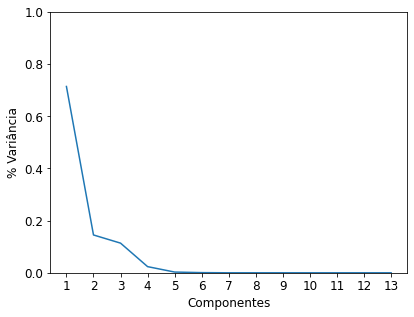
\includegraphics[scale=0.45]{images/base-de-dados-27.1-pca-components-total-secao.png}
        \caption{Percentual de variância explicada de cada componente principal}
        \label{fig:resultados:base-de-dados-27.1-pca-components-total-secao}
    \end{subfigure} ~ \quad
    \begin{subfigure}[b]{0.45\textwidth}
        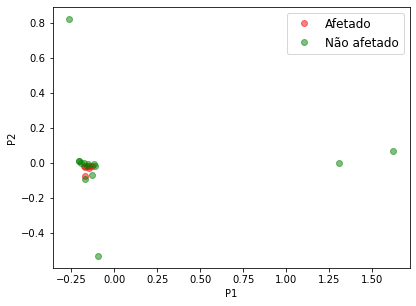
\includegraphics[scale=0.45]{images/base-de-dados-27.2-pca-2d-total-secao.png}
        \caption{Visualização dos dados projetados sobre as duas componentes principais}
        \label{fig:resultados:base-de-dados-27.2-pca-2d-total-secao}
    \end{subfigure}
    \fdadospesquisa
\end{figure}

\section{Classificação CNAE}

\begin{figure}[htb] 
    \centering 
    \caption{PCA sobre dados mensais de CNAEs}
    \label{fig:resultados:base-de-dados-28-pca-components-monthly-cnae} 
    \begin{subfigure}[b]{0.45\textwidth}
        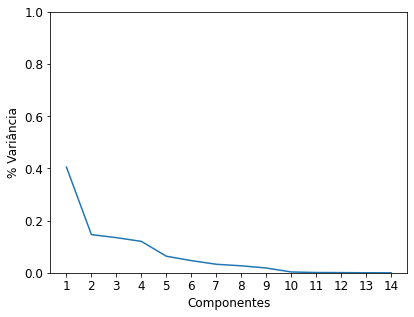
\includegraphics[scale=0.45]{images/base-de-dados-28.1-pca-components-monthly-cnae.png}
        \caption{Percentual de variância explicada de cada componente principal}
        \label{fig:resultados:base-de-dados-28.1-pca-components-monthly-cnae}
    \end{subfigure} ~ \quad
    \begin{subfigure}[b]{0.45\textwidth}
        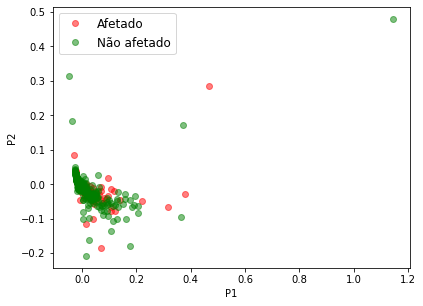
\includegraphics[scale=0.45]{images/base-de-dados-28.2-pca-2d-monthly-cnae.png}
        \caption{Visualização dos dados projetados sobre as duas componentes principais}
        \label{fig:resultados:base-de-dados-28.2-pca-2d-monthly-cnae}
    \end{subfigure}
    \fdadospesquisa
\end{figure}

\begin{figure}[htb] 
    \centering 
    \caption{PCA sobre dados totais de CNAEs}
    \label{fig:resultados:base-de-dados-28-pca-components-total-cnae} 
    \begin{subfigure}[b]{0.45\textwidth}
        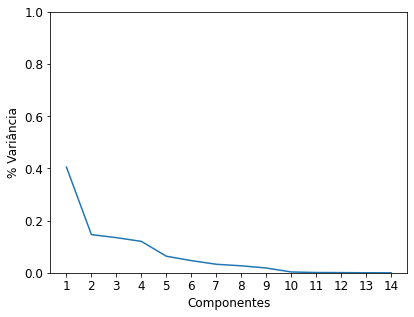
\includegraphics[scale=0.45]{images/base-de-dados-28.1-pca-components-total-cnae.png}
        \caption{Percentual de variância explicada de cada componente principal}
        \label{fig:resultados:base-de-dados-28.1-pca-components-total-cnae}
    \end{subfigure} ~ \quad
    \begin{subfigure}[b]{0.45\textwidth}
        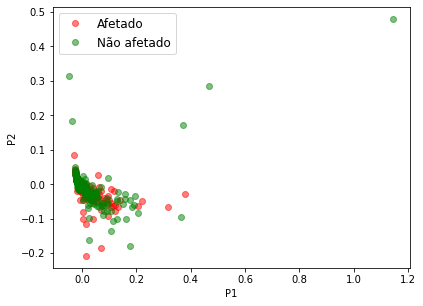
\includegraphics[scale=0.45]{images/base-de-dados-28.2-pca-2d-total-cnae.png}
        \caption{Visualização dos dados projetados sobre as duas componentes principais}
        \label{fig:resultados:base-de-dados-28.2-pca-2d-total-cnae}
    \end{subfigure}
    \fdadospesquisa
\end{figure}

\begin{figure}[htb] 
    \centering 
    \caption{Resultado tentativas de classificação para cada método aplicado sobre dados mensais de CNAE}
    \label{fig:resultados:classification-monthly-cnae} 
    \begin{subfigure}[b]{0.45\textwidth}
        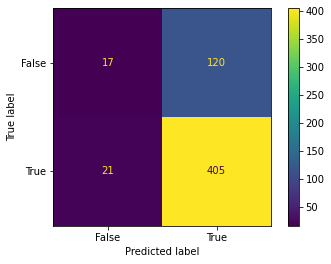
\includegraphics[scale=0.45]{images/base-de-dados-28.3.1-confusion-matrix-randomforest-monthly-cnae.png}
        \caption{Matriz de confusão para Random Forest}
        \label{fig:resultadosbase-de-dados-28.3.1-confusion-matrix-randomforest-monthly-cnae}
    \end{subfigure} ~ \quad
    \begin{subfigure}[b]{0.45\textwidth}
        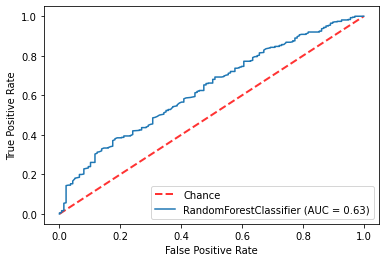
\includegraphics[scale=0.45]{images/base-de-dados-28.3.2-roc-curve-randomforest-monthly-cnae.png}
        \caption{Curva ROC para Random Forest}
        \label{fig:resultados:base-de-dados-28.3.2-roc-curve-randomforest-monthly-cnae}
    \end{subfigure} ~ \\
    \centering 
    \begin{subfigure}[b]{0.45\textwidth}
        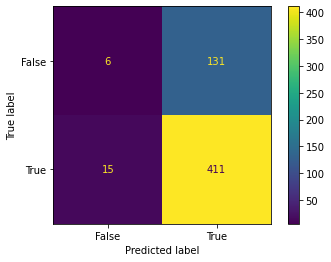
\includegraphics[scale=0.45]{images/base-de-dados-28.3.3-confusion-matrix-svc-monthly-cnae.png}
        \caption{Matriz de confusão para SVC}
        \label{fig:resultados:base-de-dados-28.3.3-confusion-matrix-svc-monthly-cnae}
    \end{subfigure} ~ \quad
    \begin{subfigure}[b]{0.45\textwidth}
        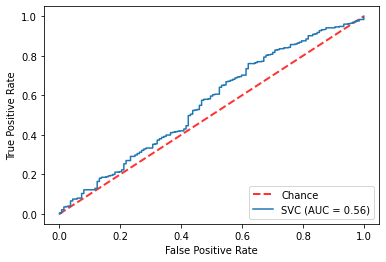
\includegraphics[scale=0.45]{images/base-de-dados-28.3.4-roc-curve-svc-monthly-cnae.png}
        \caption{Curva ROC para SVC}
        \label{fig:resultados:base-de-dados-28.3.4-roc-curve-svc-monthly-cnae}
    \end{subfigure} ~ \\
    \centering
    \begin{subfigure}[b]{0.45\textwidth}
        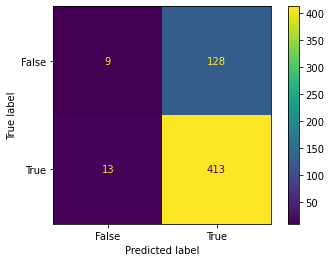
\includegraphics[scale=0.45]{images/base-de-dados-28.3.5-confusion-matrix-knn-monthly-cnae.png}
        \caption{Matriz de confusão para KNN}
        \label{fig:resultados:base-de-dados-28.3.5-confusion-matrix-knn-monthly-cnae}
    \end{subfigure} ~ \quad
    \begin{subfigure}[b]{0.45\textwidth}
        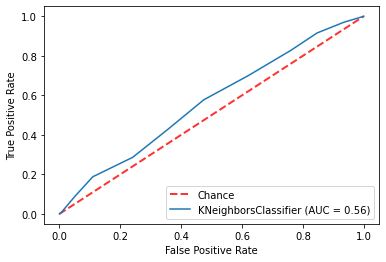
\includegraphics[scale=0.45]{images/base-de-dados-28.3.6-roc-curve-knn-monthly-cnae.png}
        \caption{Curva ROC para KNN}
        \label{fig:resultados:base-de-dados-28.3.6-roc-curve-knn-monthly-cnae}
    \end{subfigure} ~ \\
    \centering 
    \begin{subfigure}[b]{0.45\textwidth}
        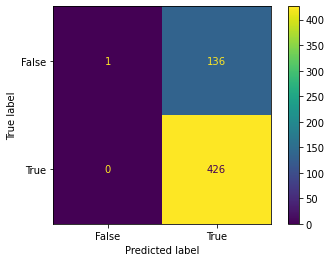
\includegraphics[scale=0.45]{images/base-de-dados-28.3.7-confusion-matrix-logregression-monthly-cnae.png}
        \caption{Matriz de confusão para Regressão logística}
        \label{fig:resultados:base-de-dados-28.3.7-confusion-matrix-logregression-monthly-cnae}
    \end{subfigure} ~ \quad
    \begin{subfigure}[b]{0.45\textwidth}
        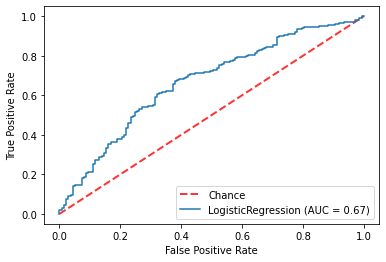
\includegraphics[scale=0.45]{images/base-de-dados-28.3.8-roc-curve-logregression-monthly-cnae.png}
        \caption{Curva ROC para Regressão Logística}
        \label{fig:resultados:base-de-dados-28.3.8-roc-curve-logregression-monthly-cnae}
    \end{subfigure} ~ \\
    \fdadospesquisa
\end{figure}

\begin{figure}[htb] 
    \centering 
    \caption{Resultado tentativas de classificação para cada método aplicado sobre dados totais de CNAE}
    \label{fig:resultados:classification-total-nae} 
    \begin{subfigure}[b]{0.45\textwidth}
        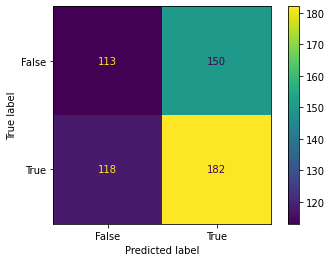
\includegraphics[scale=0.45]{images/base-de-dados-28.4.1-confusion-matrix-randomforest-total-cnae.png}
        \caption{Matriz de confusão para Random Forest}
        \label{fig:resultadosbase-de-dados-28.3.1-confusion-matrix-randomforest-total-cnae}
    \end{subfigure} ~ \quad
    \begin{subfigure}[b]{0.45\textwidth}
        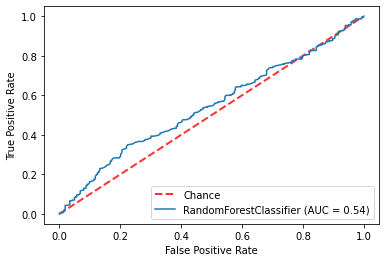
\includegraphics[scale=0.45]{images/base-de-dados-28.4.2-roc-curve-randomforest-total-cnae.png}
        \caption{Curva ROC para Random Forest}
        \label{fig:resultados:base-de-dados-28.3.2-roc-curve-randomforest-total-cnae}
    \end{subfigure} ~ \\
    \centering 
    \begin{subfigure}[b]{0.45\textwidth}
        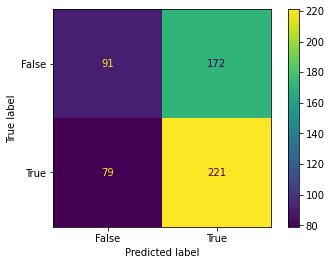
\includegraphics[scale=0.45]{images/base-de-dados-28.4.3-confusion-matrix-svc-total-cnae.png}
        \caption{Matriz de confusão para SVC}
        \label{fig:resultados:base-de-dados-28.3.3-confusion-matrix-svc-total-cnae}
    \end{subfigure} ~ \quad
    \begin{subfigure}[b]{0.45\textwidth}
        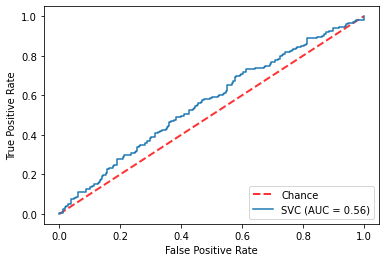
\includegraphics[scale=0.45]{images/base-de-dados-28.4.4-roc-curve-svc-total-cnae.png}
        \caption{Curva ROC para SVC}
        \label{fig:resultados:base-de-dados-28.3.4-roc-curve-svc-total-cnae}
    \end{subfigure} ~ \\
    \centering
    \begin{subfigure}[b]{0.45\textwidth}
        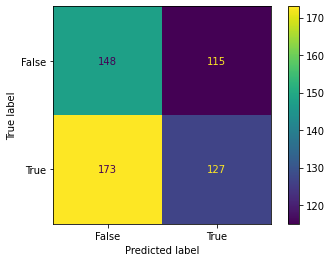
\includegraphics[scale=0.45]{images/base-de-dados-28.4.5-confusion-matrix-knn-total-cnae.png}
        \caption{Matriz de confusão para KNN}
        \label{fig:resultados:base-de-dados-28.3.5-confusion-matrix-knn-total-cnae}
    \end{subfigure} ~ \quad
    \begin{subfigure}[b]{0.45\textwidth}
        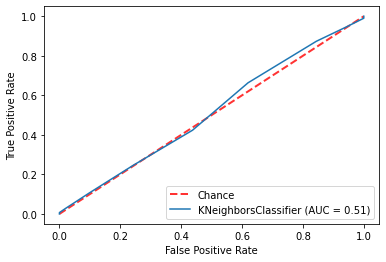
\includegraphics[scale=0.45]{images/base-de-dados-28.4.6-roc-curve-knn-total-cnae.png}
        \caption{Curva ROC para KNN}
        \label{fig:resultados:base-de-dados-28.3.6-roc-curve-knn-total-cnae}
    \end{subfigure} ~ \\
    \centering 
    \begin{subfigure}[b]{0.45\textwidth}
        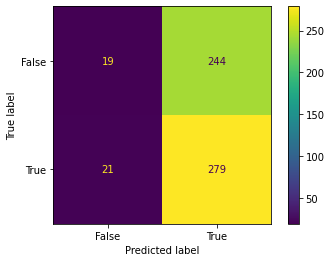
\includegraphics[scale=0.45]{images/base-de-dados-28.4.7-confusion-matrix-logregression-total-cnae.png}
        \caption{Matriz de confusão para Regressão logística}
        \label{fig:resultados:base-de-dados-28.3.7-confusion-matrix-logregression-total-cnae}
    \end{subfigure} ~ \quad
    \begin{subfigure}[b]{0.45\textwidth}
        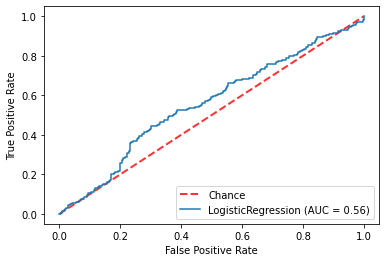
\includegraphics[scale=0.45]{images/base-de-dados-28.4.8-roc-curve-logregression-total-cnae.png}
        \caption{Curva ROC para Regressão Logística}
        \label{fig:resultados:base-de-dados-28.3.8-roc-curve-logregression-total-cnae}
    \end{subfigure} ~ \\
    \fdadospesquisa
\end{figure}
